 \section{Multi Label Learning}
 
\subsection*{Introduction}
\begin{frame}{Multi label classification}
	Motivation:
	\begin{itemize}\setlength\itemsep{1em}
		\item Sometimes a complex item can be well represented by a set of \textit{labels}
		\item Helps single label classification when the concept is more complicated or general
	\end{itemize}
	Solutions \cite{ml_approaches}:
	\begin{itemize}\setlength\itemsep{1em}
		\item Problem transformation
		\item Algorithm adaptation
	\end{itemize}
\end{frame}

\begin{frame}{Notation}
	A set of labels $L = \{y_1, y_2,... y_l\}$ is given.\\
	Each object contained in the dataset is associated with a set of labels:
	\begin{columns}
		\begin{column}{0.5\textwidth}\centering
		$$D = \{(X_i, Y_i | i \in [1, n]\}$$
		$$X_i \in \R^f$$
		$$Y_i = \{y_{i,h} | h \in [1, h_i], y_{i,h} \in L, h_i \leq l\}$$
		\end{column}
		\begin{column}{0.5\textwidth}\centering
		\begin{figure}[htbp]
			\centering
			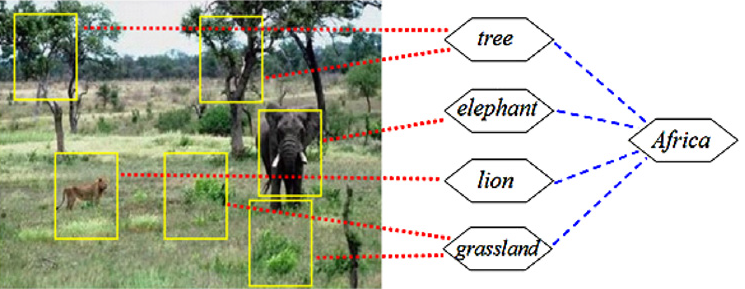
\includegraphics[scale = 0.3]{./images/ml1.png}
			\caption{\textit{Multi label example}}
		\end{figure}
		\end{column}
	\end{columns}
	
\end{frame}

\begin{frame}{Problem transformation}
	Attempt to convert the multilabel problem in a regular binary task.
	
	Two lossy methods:
	\begin{itemize}\setlength\itemsep{1em}
		\item Randomly discard each label information except one from each instance
		\item Remove instances that have actually more than one label
	\end{itemize}
	Other solutions:
	\begin{itemize}\setlength\itemsep{1em}
		\item Train a binary classifier for each existing combination of labels
		\item Train a binary classifier for each label (used in this work)
	\end{itemize}
\end{frame}

\begin{frame}{An algorithm adaptation approach}
	The idea is to focus on ranking rather than binary classification \cite{ml1}

	\begin{itemize}
		\item Train a classifier $f_l : X \rightarrow \mathbb{R}$ for each label
		\item For each test example sort label list according to predicted rank
		\item Set size prediction feeding dataset and thresholds $t(X_i)$ to a classifier
		$$t(X_i) = argmin_t\{ k \in Y_i \ s.t. \ f_k(X_i) \leq t \} + \{ k \in \bar{Y}_i \ s.t. \ f_k(X_i) \geq t \}$$
		\item Take the best labels according to set size prediction:
	\end{itemize}
	
\end{frame}